\documentclass[tikz]{standalone}
\usetikzlibrary{arrows, positioning}
\tikzset{
  treenode/.style = {align=center, inner sep=1pt, text centered,
    font=\sffamily},
  arn_b/.style = {treenode, circle, white, font=\sffamily\bfseries, draw=black,
    fill=black, text width=2em},% arbre rouge noir, noeud noir
  arn_r/.style = {treenode, circle, red, draw=red, 
    text width=2em, very thick},% arbre 
  arn_a/.style = {treenode, circle, white, fill=brown, draw=brown, 
    text width=2em, very thick}% arbre  
}

\begin{document}
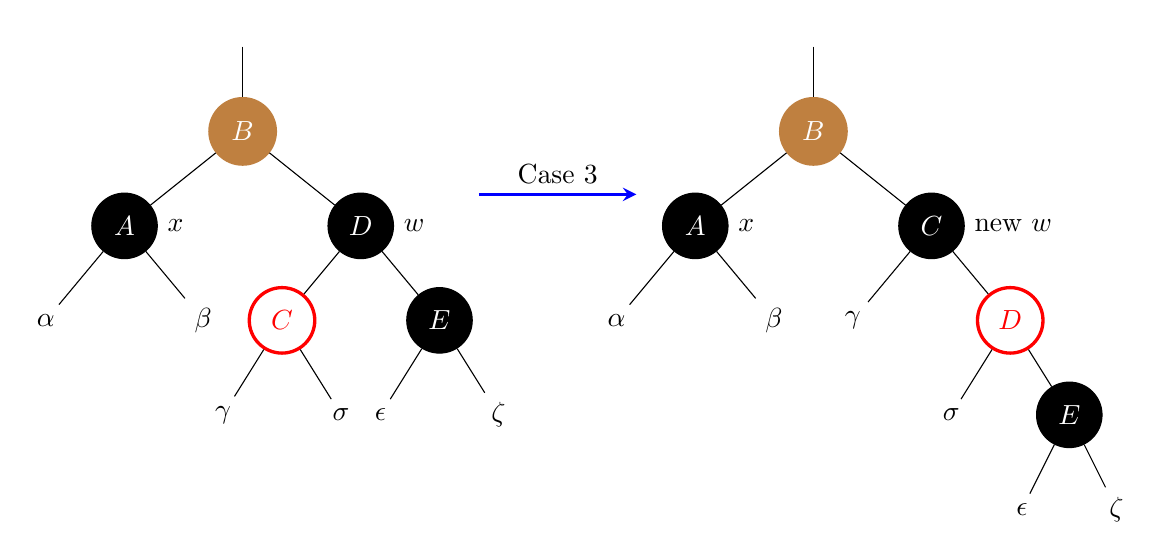
\begin{tikzpicture}[level/.style={sibling distance = 6cm/#1,
    level distance = 1.2cm}]
    \node (lefttree) {}
        child {node [arn_a] {$B$}
            child {node (1na) [arn_b] {$A$}
                child{node {$\alpha$}}
                child{node {$\beta$}}
            }
            child {node (1nd) [arn_b] {$D$}
                child {node [arn_r] {$C$}
                    child {node {$\gamma$}}
                    child {node {$\sigma$}}
                }
                child {node [arn_b] {$E$}
                    child {node {$\epsilon$}}
                    child {node {$\zeta$}}
                }
            }
        }
    ;
    \node [right] at (1na.east) {$x$}; 
    \node [right] at (1nd.east) {$w$}; 
    
    \draw [-stealth, line width=0.4mm, draw=blue](3,-2) -- (5,-2)node[midway,above,shape=rectangle,draw=none]{Case 3};
    
    \node (righttree) [right=of lefttree, xshift=6cm] {}
    child {node [arn_a] {$B$}
        child {node (2na) [arn_b] {$A$}
            child{node {$\alpha$}}
            child{node {$\beta$}}
            }
        child {node (2nc) [arn_b] {$C$}
            child {node {$\gamma$}}
            child {node [arn_r] {$D$}
                child {node {$\sigma$}}
                child {node [arn_b] {$E$}
                child {node {$\epsilon$}}
                child {node {$\zeta$}}
                }
            }
        }
    }
;
\node [right] at (2na.east) {$x$}; 
\node [right] at (2nc.east) {new $w$}; 
\end{tikzpicture}
\end{document}